\subsection*{Hjørner}\label{subsec:corner}
Et hjørne kan defineres som et område i og omkring et punkt, der har to dominerede kantretninger. I figur \ref{app} ses tre udvalgte punkter, placeret forskellige steder i samme scene. Punkterne beskrives ud fra den information, der indgår i den mørkeblå cirkel, omkring punktet. Punkter placeret på hjørner, kan bruges som interessepunkter. Dette kan vises igennem de tre billeder opstillet nedenfor.
\begin{enumerate}[label=\alph*]
\item{Interessepunktet er placeret på et fladt området, hvor intensiteten er ens for hele området. Punktet vil have mange mulige korresponderende punkter.}
\item{Interessepunktet er lokaliseret på en gul kant. Punktet vil have flere mulige korresponderende punkter på den tilsvarende kant i den anden figur.}
\item{Interessepunktet er lokaliseret på et hjørne. Det ses at kun ét andet punkt i modsvarende scene er identisk med dette.}
\end{enumerate}
\begin{figure}[H]
    \centering
    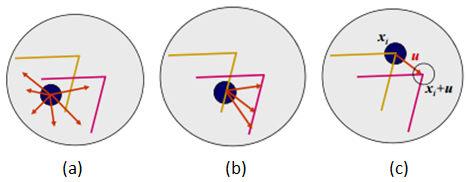
\includegraphics[width=0.75\textwidth]{fig/37.png}
    \vspace{-1em}   
    \begin{center}    
    \caption{{\footnotesize \textit{Tre interessepunkter placeret forskelligt i en scene. Interessepunkterne er placeret: (a) på et fladt område (b) på en kant (c) på et hjørne. 
 }}}
    \label{app}
     \end{center}
    \vspace{-2.7em}  
  \end{figure}  
\noindent
Ovenstående viser at punkter placeret på hjørner unikt kan skelnes fra andre punkter. 